% Chapter 4
% ======================================================================================================
% NOTES, TODOS

% ======================================================================================================

\chapter{Experiment}
\label{Chapter4} % For referencing the chapter elsewhere, use \ref{Chapter1} 

The primary objective of this research is to demonstrate the feasibility of using lightweight encryption/authentication with new proposed  schemes to improve communication security between constrained devices and Digital Twin. To validate the efficacy of our proposed solution, we conducted experiments using an ESP32 as the constrained device candidate and a widely-used open-source digital twin platform called Ditto. This section provides a comprehensive overview of the experimental setup (see Fig \ref{fig:experiment-setup}) used in this study and detailed implementation specifications for the lightweight encryption/authentication algorithm implemented on both the constrained device and the digital twin platform.

\begin{figure}[H]
    \caption{Research Experiment Setup}
    \centering
    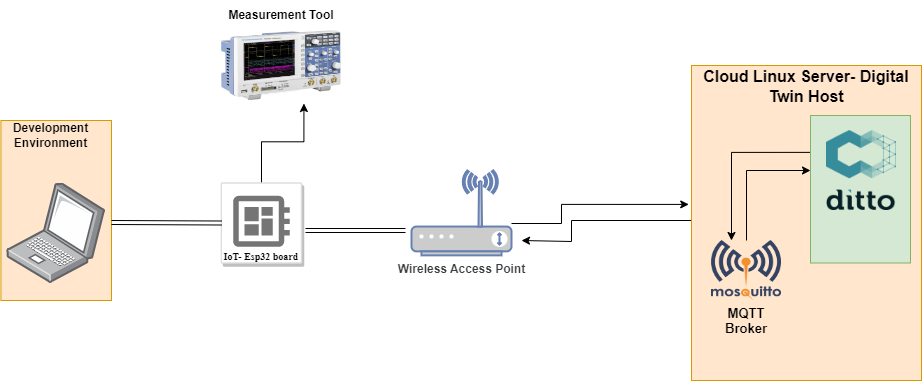
\includegraphics[width=\textwidth]{images/fp/experiment.drawio.png}
    \label{fig:experiment-setup}
\end{figure}



\section{Wemos Lolin32 Lite}

The Wemos LOLIN32 Lite is a low-cost, low-power system on a chip (SoC)  microcontroller that is popular for Internet of Things (IoT) projects. It is based on the ESP32 SoC, which has a 32-bit dual-core processor, 4MB of flash memory, and 520kB of RAM. The LOLIN32 Lite also has Wi-Fi and Bluetooth connectivity, making it ideal for this projects for sending and receiving data to and from Digital Twin through a wireless connection.


% \begin{figure}[H]    
%     \caption{}
%     % \centring
%     \begin{subfigure}[b]{0.45\textwidth}
%     \caption{Number of selected papers per publisher.}
       
        
%     \end{subfigure}
%     \begin{subfigure}[b]{0.45\textwidth}
%     \caption{Number of selected papers per source.}
       
%     \end{subfigure}
%     \label{fig:esp32}
% \end{figure}



\begin{figure}[ht]
  \centering
  \begin{minipage}{0.5\textwidth}
    \centering
    \caption{Temporary Image Replacement for ESP32 board}
    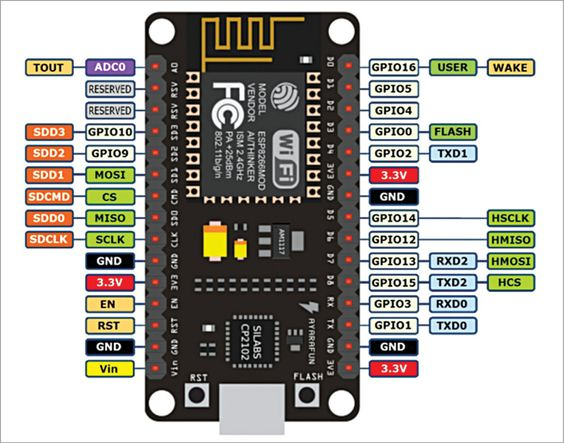
\includegraphics[width=\textwidth]{images/fp/ESP32.jpg}
    \label{fig:example-image}
  \end{minipage}%
  \hspace{0.2cm}
  \begin{minipage}{0.45\textwidth}
    \centering
    \begin{table}[H]
        % \tiny
        \centering
        \caption{\label{tbl:esp-spec} Technical Specification of Wemos Lolin32 Lite}
        % \resizebox{\linewidth}{!}{
        \begin{NiceTabular}{|p{2.5cm}|p{3cm}|}
        \CodeBefore
        % \rowcolors[gray]{2}{0.8}{}[cols=1-2,restart]
        \Body
        \toprule
        	Operating voltage &  3.3V \\
            \hline
        	Supported Battery &	Lipo 3.7V\\
            \hline
        	Battery Connector & PH-2 2.0mm\\
            \hline
        	Digital I/O Pins & 22 \\
            \hline
        	 RAM Memory &  512KB\\
            \hline
            Clock Speed(Max) &	240MHz \\
            \hline
            SPI Flash &	4M Bytes \\
            \hline
            Size & 57*25.4mm \\
        \bottomrule
        \end{NiceTabular}
        % }
    \end{table}
  \end{minipage}
\end{figure}

One of the key advantages of the Wemos LoLin32 Lite board is that it is supported by both the Arduino and ESP-IDF (Espressif IoT Development Framework) development environments. For our research project, we opted to use the Arduino embedded development framework in order to implement the ASCON and AES-GCM algorithms using the C and C++ programming languages. In addition, we utilized PlatformIO, an open-source platform for embedded development, to facilitate the building and deployment of our program onto the Wemos LoLin32 Lite board via the serial port.

% ======================================================================================================
% NOTES, TODOS
% What is Ditto -> reference the official webisite

% ======================================================================================================

\section{Eclipse Ditto - Digital Twin Setup}
Eclipse Ditto is an open-source framework that provides a way to create and manage Digital Twin of connected devices [ref]. Ditto can be deployed on-premises or in the cloud. For this research, we build and deploy the ditto code base using docker on a virtual private cloud server. 


We have two options for deploying and running Ditto on a cloud Linux server. The first option involves utilizing the Kubernetes cluster, which necessitates substantial infrastructure resources. Specifically, a minimum of 4 GB RAM, 8 core processes, and 20 GB disk storage are required. However, the second option, which we have chosen, involves using Docker. This alternative demands fewer resources compared to the previous one. Under this option, we have seven microservices operating in parallel, each fulfilling distinct functions. These microservices include Nginx as the web server, Ditto Gateway, Ditto Connectivity for managing the device-to-Ditto connectivity, Ditto Thing for overseeing things (representing physical devices), Thing Search for facilitating efficient search using MongoDB, Swagger-UI for providing a web-based user interface, and Ditto Policies for access control on things.

The following steps outline the process required to set up Ditto on a Linux server:

\begin{itemize}
    \item Step 1: Install and configure the Docker demon including the docker composer utility.
    \item Step 2: Clone the Eclipse Ditto code base from the official GitHub page using the command: \texttt{git clone https://github.com/eclipse-ditto/ditto.git}
    \item Start running the Ditto cluster as microservices in a container by executing the command: \texttt{docker-compose up -d}
    \item Verify that all microservices are running and check the health status of Ditto using the following commands: \texttt{curl -u devops:foobar\\ http://localhost:8080/status/health}
\end{itemize}
The process of running Ditto and connecting with the MQTT broker is described below.

\textit{Creating Policy}: In Ditto policies are JSON configuration file that defines who access what. Creating policies is the first step in running Ditto. The policy configuration we use for our project is presented as follows. To speed up experimenting with Ditto we used a bash script that we can run from the terminal of the server. 
\begin{lstlisting}[style=CStyle]
#!/bin/bash

curl -X PUT 'http://localhost:8080/api/2/policies/ut.thesis.demo:policy' -u 'ditto:ditto' -H 'Content-Type: application/json' -d '{
    "entries": {
        "owner": {
            "subjects": {
                "nginx:ditto": {
                    "type": "nginx basic auth user"
                }
            },
            "resources": {
                "thing:/": {
                    "grant": [
                        "READ","WRITE"
                    ],
                    "revoke": []
                },
                "policy:/": {
                    "grant": [
                        "READ","WRITE"
                    ],
                    "revoke": []
                },
                "message:/": {
                    "grant": [
                        "READ","WRITE"
                    ],
                    "revoke": []
                }
            }
        }
    }
}'

\end{lstlisting}

\textit{Creating things}: Things are the digital representation of the physical device with attributes and features. Like we did for policy, for the thing we also created bash script as follow. 

\begin{lstlisting}[style=CStyle]
    

#!/bin/bash

curl -X PUT 'http://localhost:8080/api/2/things/ut-sensors:esp01' -u 'ditto:ditto' -H 'Content-Type: application/json' -d '{
    "policyId": "ut.thesis.demo:policy",
    "attributes": {
        "name": "Esp3201",
        "type": "Esp32 board"
    },
    "features": {
        "temperature": {
            "properties": {
                "value": 0
            }
        },
        "altitude": {
            "properties": {
                "value": 0
            }
        }
    }
}'
\end{lstlisting}

\textit{Creating connection:} The connection configuration file serves the purpose of defining the source and target of the MQTT broker topic. In this case, the connection type is MQTT, and the specified URI contains the IP address. The source topic is set as "ut-sensors/\#", indicating that Ditto will receive data from the broker when a message is published on any topic under "ut-sensors". On the other hand, the target address is defined as "ut-sensors/{{thing:id}}", which means that Ditto will publish data on the corresponding topic of the device whenever an event is emitted by the thing with the given ID. The inclusion of "\#" at the end of the string signifies that messages can be received from any topic under "ut-sensors". This configuration enables bidirectional communication and data exchange between Ditto and IoT devices via the MQTT broker. 

\begin{lstlisting}[style=CStyle]
#!/bin/bash

curl -X POST 'http://localhost:8080/devops/piggyback/connectivity?timeout=10' -u 'devops:foobar' -H 'Content-Type: application/json' -d '{
    "targetActorSelection": "/system/sharding/connection",
    "headers": {
        "aggregate": false
    },
    "piggybackCommand": {
        "type": "connectivity.commands:createConnection",
        "connection": {
            "id": "ascon-ut-mqtt-connection",
            "connectionType": "mqtt",
            "connectionStatus": "open",
            "failoverEnabled": true,
            "uri": "tcp://<IP address>:1883",
            "sources": [{
                "addresses": ["ut-sensors/#"],
                "authorizationContext": ["nginx:ditto"],
                "qos": 0,
                "filters": [],
                                "headerMapping": {},
                                "payloadMapping": ["AsconPayload"],
                                "replyTarget": {
                                        "headerMapping": {},
                                        "expectedResponseTypes": [
                                          "response",
                                          "error"
                                        ],
                                        "enabled":false
                                }
            }],
                        "targets": [{
                                "address": "ut-sensors/{{ thing:id }}",
                                "topics": [
                                "_/_/things/twin/events",
                                "_/_/things/live/messages"
                                ],
                                "authorizationContext": ["nginx:ditto"],
                                "headerMapping": {},
                "qos": 0,
                "payloadMapping": ["AsconPayload"]
                        }]
        }
    }
}'
\end{lstlisting}


The other important component of Ditto that works hand in hand is MQTT broker. In the following section we provide detail of how setup it and start running. 

Another crucial component that works hand in hand with Ditto is the MQTT broker. In the subsequent section, we will deep dive into the detailed process of setting it up and initiating its operation.

\section{Building MQTT Broker (Mosquitto) from Source}

The MQTT broker is a lightweight protocol designed for IoT communication[ref]. In our project, we utilized the MQTT implementation from Eclipse Ditto, specifically Mosquitto. To ensure full control and customization, we built the MQTT implementation from the source on our Linux server. This approach was undertaken primarily to accommodate the implementation of the lightweight encryption algorithm into the source code. However, we later decided to implement the algorithms by extending the ditto source code itself through the connectivity extension provided. 

In order to run the MQTT broker on our Linux server, there are a few necessary steps to follow. Firstly, we need to install a couple of dependencies, namely \texttt{libcjson-dev and libwebsocket-dev}. Once these dependencies are installed, we proceed to build the source code by executing the following command: \texttt{make WITH\_SRV=yes WITH\_TLS=no WITH\_WEBSOCKETS=yes WITH\_CJSON = yes WITH\_BUNDLED\_DEPS = yes WITH\_DOCS=no}. After the build process, we can verify the successful installation of MQTT by running the tests using the command \texttt{make test}. Finally, to complete the installation, we execute \texttt{sudo make install} to install the MQTT broker into our system. 


It is worth noting that the MQTT broker can be installed either on the same machine as the Ditto running machine or on a different remotely accessible machine. Our proposed scheme ensures secure communication between the IoT device and the cloud-hosted Ditto service. The MQTT broker has limited visibility, as it can only access the encrypted payload, thereby preventing any malicious broker from compromising the security of the communication. The lightweight authentication and encryption algorithm we leverage into our proposed solution guarantees the confidentiality and integrity of the data exchanged.

To start the MQTT service, there are two options available. The first option is to execute the command "mosquitto" directly. Alternatively, we can start the MQTT service with additional configuration options by specifying the configuration file path using the following command: "mosquitto -v -c /path/to/mosquitto.conf".

To publish and subscribe to topics using the MQTT broker, we utilize the commands provided on the GitHub page of Mosquitto. 
    \begin{itemize}
        \item For subscribing to a topic, we employ the command "mosquitto\_sub -t 'test/topic' -v". This command enables us to subscribe to the specified topic and receive the messages associated with it. 
        \item To publish a message to a topic, we run "mosquitto\_pub -t 'test/topic' -m 'hello world'". By executing this command, we can publish a message to the specified topic so that other subscribers to the topic get notified. 
    \end{itemize}
    
    
% \begin{figure}[H]
%     \caption{Ditto Architecture}
%     \centering
%     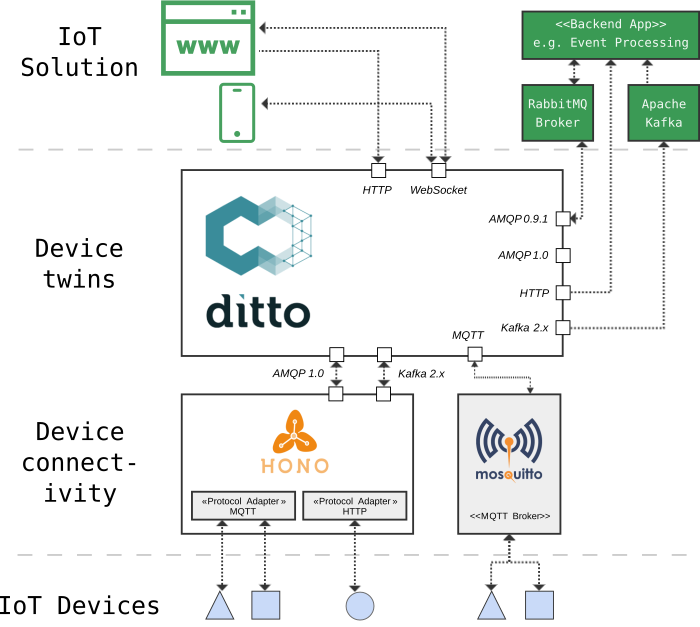
\includegraphics[width=\textwidth]{images/fp/ditto-overview-1.png}
%     \label{fig:ditto-arch}
% \end{figure}




\section{Implementation of ASCON and AES-GCM for device}





The implementation of both algorithms on the hardware IoT device was carried out using C and C++ programming languages within Arduino for esp-idf embedded development framework. We opted for C and C++ because those two choices are more suitable for low-level programming such as for embedded resource constraint devices. The main application for the IoT device was developed in C++, while the algorithm for ASCON and AES-GCM was implemented in C and incorporated through the use of the "extern" macro in C++ main application.


The counterpart of the algorithms in the digital twin was implemented in Java. This is because the connectivity microservice of Ditto is implemented in Java. This allowed us to extend the connectivity module using Java to incorporate an extension for encryption and decryption of the payload that comes from IoT devices.

It is important to note the implementation for each algorithm (ASCON\footnote{https://github.com/ascon/ascon\_collection} and AES-GCM\footnote{https://github.com/usnistgov/Lightweight-Cryptography-Benchmarking/tree/main/implementations/\_reference\_/crypto\_aead/aes-gcm/mbedtls}) was done using the reference implementation from their respective GitHub page, without introducing any optimization or modifications.


\section{MQTT Payload Encryption/Authentication }

In Chapter 6, payload encryption was discussed as a means of ensuring message confidentiality at the application level. This approach can be used to establish an end-to-end secure channel between the sender and receiver at the application level  to provide confidentiality over transmitted data. However, in this paper, we extend the scope beyond message confidentiality and introduce the ASCON algorithm to provide both message authenticity and confidentiality.

Furthermore, in this paper, we use the device id as associative or additional data used along the key and plain text as input for the implementation of the ASCON and AES-GCM algorithms. It is important to highlight that the device ID and its corresponding private key are assumed to be pre-shared between the communicating parties prior to initiating communication. In our case, while the device id is managed and maintained by the Digital Twin device registration module, the symmetric key should be explicitly configured from both side of the implementtion.  

The MQTT protocol is a lightweight messaging protocol that is often used in the Internet of Things (IoT). MQTT protocol can be configured and programmed to supports payload encryption using any encryption algorithm, including the ASCON and AES-GCM. 


\begin{figure}[H]
    \caption{Scheme of Payload Encryption With Authentication Over MQTT Protocol. }
    \centering
    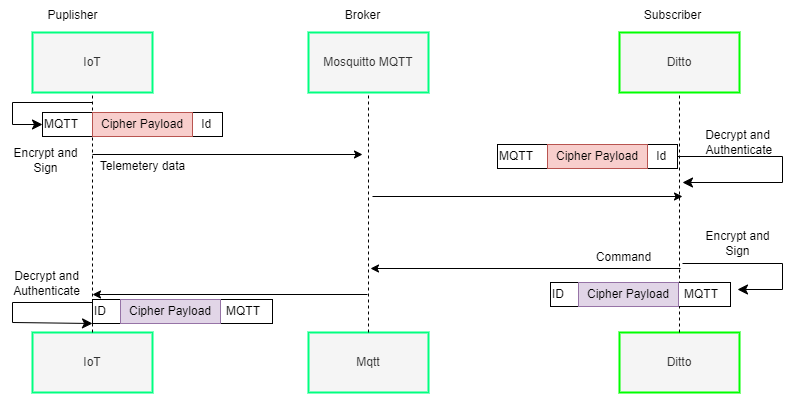
\includegraphics[width=\textwidth]{images/fp/payloadenc.drawio.png}
    \label{fig:payload-encauth-schem}
\end{figure}

To achieve payload encryption using ASCON or AES-GCM algorithm over the MQTT protocol, the following steps should be taken. 
\begin{itemize}
    \item[-] \textit{Device ID registration}: Each connected device to Ditto should have a unique device id. 
    \item[-] \textit{Generate and manage encryption keys}: The device and the Digital Twin agree on a symmetric key. 
    \item[-] \textit{Encryption and Sending a message}: The sender encrypts the payload of the message along with a tag generated and publishes it to the MQTT broker. In this case, associated data is the unique id of the device sending and receiving data to and from the Digital Twin. 
    \item[-] \textit{Forwarding or Proxing}: The MQTT broker proxies the message through the publisher-subscriber setting. 
    \item[-] \textit{Decryption and Authentication}: The receiver (subscriber) receives the MQTT message and decrypts and authenticates the payload using the agreed key and claimed device ID.
    
\end{itemize}


\subsection{End-To-End Encryption and Authentication}
Our communication scheme based on payload encryption and authentication using one of the AEAD (authenticated encryption with associated data) algorithms over the MQTT protocol implicitly provides end-to-end confedentiality and integrity of a communicated message. The Mosquitto broker acts as a proxy for forwarding encrypted payload messages, which are eventually decrypted and authenticated by the receiving application. 


\section{Ditto Java Base Payload Mapping}

In the context of Eclipse Ditto, data storage and transfer are facilitated through a format known as the Ditto protocol. This protocol utilizes a JSON structure, employing key-value pairs to represent and transmit information.

To seamlessly integrate with Ditto's capabilities, the connectivity microservice bundled with Ditto offers an extension specifically designed for intercepting incoming data. This extension allows for the mapping of data from its original form to a format that Ditto can understand and store in its underlying MongoDB database. Using the Ditto payload mapping feature, we can decrypt incoming encrypted payload messages and convert them into a format that Ditto can process and store.
 
With the payload mapping feature in Ditto's connectivity microservice, we can do the following: receive encrypted data from the IoT device, decrypt and authenticate it, and convert it into Ditto protocol messages. This helps ensure that the data sent between the IoT device and Ditto is secure and authentic.

To implement our custom mapping functionality to encrypt and decrypt, we perform the following steps:
\begin{itemize}
    \item[-] Implement and build a Java class as Jar file for the encryption and decryption functionality. This class will provide the ASCON or AES-GCM encryption and decryption operations needed for secure communication and data handling. 
    \item[-] Develop a custom message mapper class that will handle the conversion of incoming device messages to the appropriate Ditto protocol format. This class will integrate with the aforementioned encryption and decryption functionality to ensure data integrity and security during the mapping process.
    \item[-]Configure the Ditto connectivity microservice to recognize and load our custom message mapper. This configuration step ensures that incoming messages are routed to our custom mapper for processing, enabling seamless integration of our specific data transformation requirements within the Ditto framework.
\end{itemize}









\section{Sending Authenticated Encrypted Payload To Ditto}

This section demonstrates the proof of concept securing the communication between the IoT device and the Digital Twin (Ditto). 

Figure \ref{fig:log-mon} depicts a snapshot captured from the serial monitor output of the board (device) utilizing PlatformIO (embedded development framework). The image showcases the device transmitting an encrypted payload to the 'ut-sensors' topic while including additional data labeled as 'tid' to uniquely identify the device. In Figure \ref{fig:wireshark}, a captured packet during the communication is displayed. Upon observation, it becomes evident that the topic being utilized is 'ut-sensors', and the message section of the MQTT protocol header contains the device identifier along with the encrypted payload.


\begin{figure}[H]
    \caption{Serial Monitor of ESP32 Board and Wireshark Capturing Communication Between The Device and Ditto(DT)}
    \begin{subfigure}[c]{1\linewidth}
        \centering
        \caption{Log Output of ESP32 Device Using Serial Monitor}
        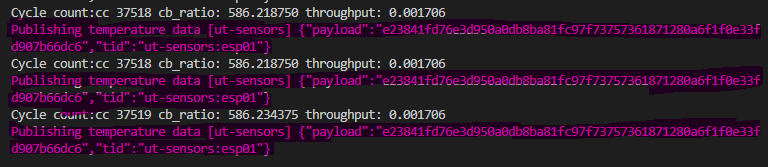
\includegraphics[width=\linewidth]{images/fp/serialport.png}
        \label{fig:log-mon}
     \end{subfigure}    

    \begin{subfigure}[c]{1\linewidth}
        \centering
        \caption{Wireshark Captured MQTT Communication From IoT to Ditto}
        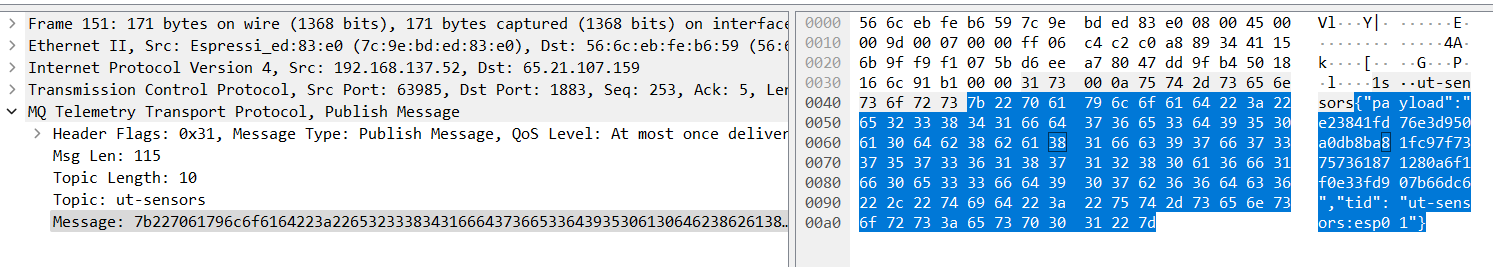
\includegraphics[width=\linewidth]{images/fp/wireshark.png}
        \label{fig:wireshark}
    \end{subfigure}
\end{figure}

The MQTT broker, hosted on the same server  with Ditto, acts as a proxy, facilitating the transmission of authenticated and encrypted payloads through a publish-subscribe model. Once the MQTT broker receives a payload, it  notifies Ditto of the new message it has subscribed to. Ditto then retrieves the payload, decrypts it, and maps it into a Ditto protocol message, which is subsequently stored in a database.

To simulate the life cycle of a Digital Twin, we have developed a small web application that models the temperature and humidity features of an ESP32 sensor. The application utilizes JavaScript to retrieve these values through a stream of emissions using server-side events (SSE). Moreover, to send commands or messages to the server, we employ the HTTP POST API of Ditto. By subscribing to the command event associated with a specific topic, any device can consume the message and execute the corresponding action. This activity effectively simulates the communication between the digital twin and the actuators. Conversely, the communication from the IoT device to the Digital Twin serves the purpose of collecting telemetry data from the operational environment.

Figure \ref{fig:ditto-log} illustrates the WebUI of Ditto, which is included by default in the code base. This web portal serves as a portal offering device, policy, and connection management functionalities. Additionally, Figure \ref{fig:appdt} provides an overview of an application layer built on the Digital Twin concept. The attributes displayed on the upper part of the image represent the name and type of the simulated device. The gauges visually represent the received device features, while the bottom right section presents textual information associated with the device.
 
\begin{figure}[H]
    \caption{Ditto and Webapp Toward Simulating Digital Twin}
    \label{fig:ditto-app}
    \begin{subfigure}[c]{1\linewidth}
        \caption{A Data Log Viewed from Ditto Platform}
        \centering
        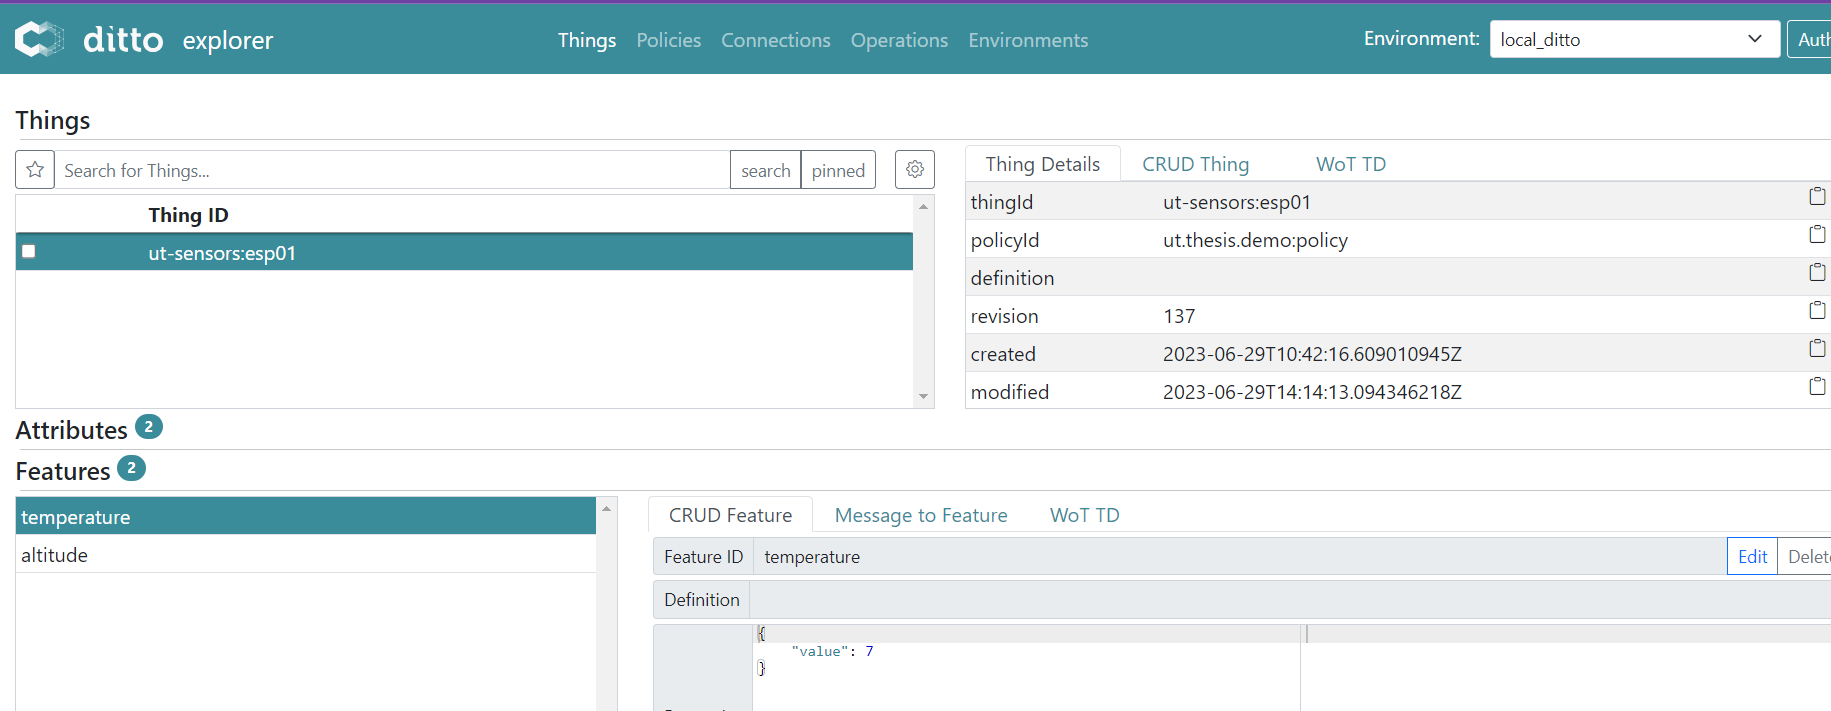
\includegraphics[width=\linewidth]{images/fp/ditto-log.png}
        \label{fig:ditto-log}
    \end{subfigure}
    
    \begin{subfigure}[c]{1\linewidth}
        \centering
        \caption{Web Application For Modeling Temperature and Humidity of ESP32}
        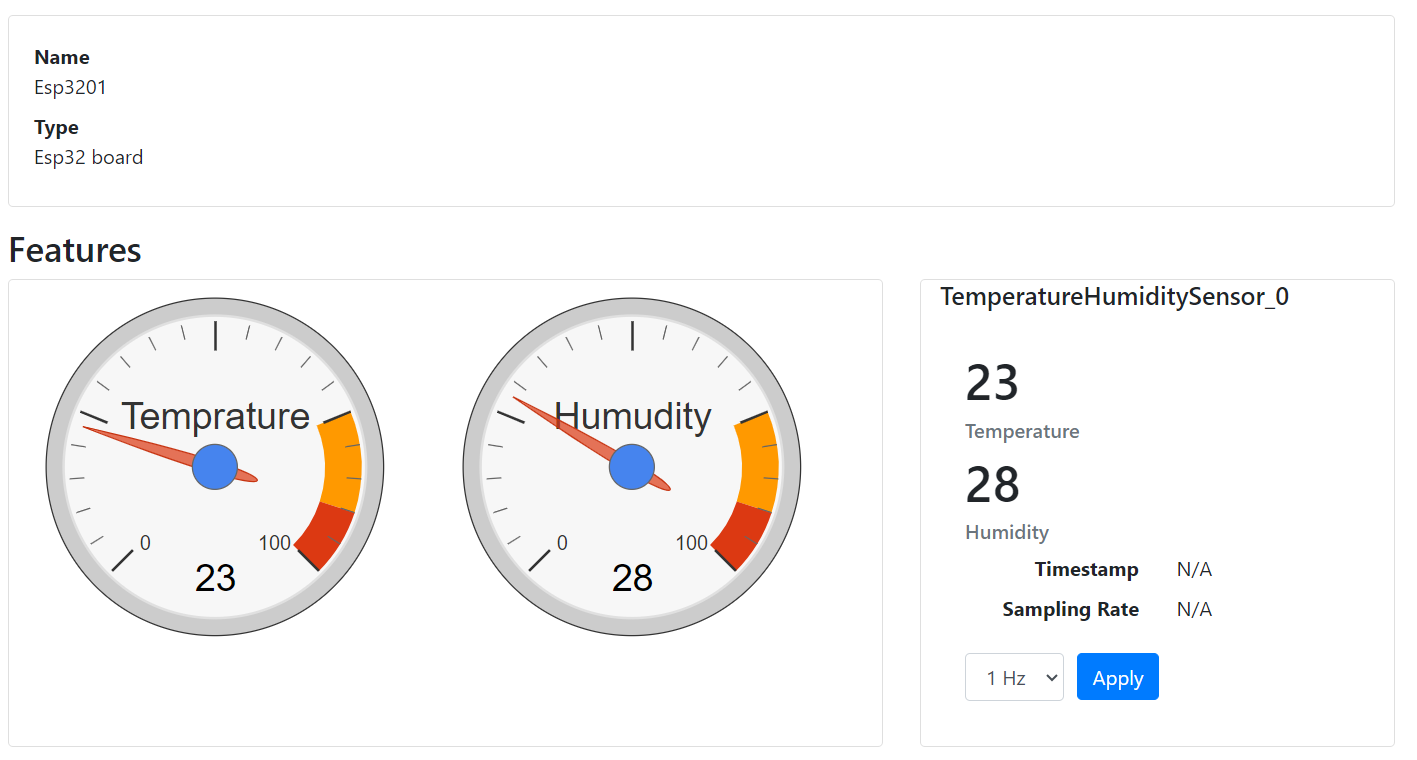
\includegraphics[width=\linewidth]{images/fp/appgauge.png}
        \label{fig:appdt}
     \end{subfigure}    
\end{figure}

\section{Performance Evaluation and Analysis}


The performance analysis section of this paper aims to measure and evaluate the power consumption, latency, and memory usage of the algorithms employed in the proposed scheme.

To measure the performance of our proposed solution, we prepared six case scenarios, which were categorized into two groups. The first group of three cases measured the performance from an algorithm perspective, while the second group of three cases measured the performance from a running application perspective.


\textit{Case 1: AES-GCM} - For this case, we use the AES-GCM encryption function to pass a plain text message and received encrypted and authenticated cipher text. 

\textit{Case 2: ASCON} - 
Unlike Case 1, the ASCON encryption function is employed to encrypt the message in this scenario.

\textit{Case 3: No encryption} - This case scenario was used as a baseline reference for the other two cases. In this case, we called a function that has a similar signature to the encryption function calls we used for ASCON and AES-GCM. However, the underlying function did not perform any operation other than copying values from one memory to another. The implementation code for this case can be seen in the following code list.

\begin{lstlisting}[style=CStyle]
int crypto_aead_encrypt(
      unsigned char *c,unsigned long long *clen,
      const unsigned char *m,unsigned long long mlen,
      const unsigned char *ad,unsigned long long adlen,
      const unsigned char *nsec,
      const unsigned char *npub,
      const unsigned char *k
      )
{
  *clen = mlen + CRYPTO_ABYTES;
  memcpy(c, m, mlen);
  memset(c + mlen, 0, CRYPTO_ABYTES);

  return 0;
}

int crypto_aead_decrypt(
  unsigned char *m, unsigned long long *mlen,
  unsigned char *nsec,
  const unsigned char *c, unsigned long long clen,
  const unsigned char *ad, unsigned long long adlen,
  const unsigned char *npub,
  const unsigned char *k
)
{
  unsigned long long len = *mlen = clen - CRYPTO_ABYTES;
  memcpy(m, c, len);

  return 0;
} 
\end{lstlisting}


\subsection{Speed - Running Time}
% execution time 
% 
In the Arduino ESP-IDF framework, we measure the execution time of a function using the built-in functions provided by the framework. The \texttt{esp\_timer\_get\_time()} function is used to retrieve the current time in microseconds since the underlying device boot. By capturing the start time before executing the function and the end time after the function completes, we calculate the execution time by subtracting the start time from the end time.

Our experimental setup involves three distinct case scenarios. Firstly, we measure the execution time when the application runs without any encryption algorithm. Then, we measure the execution time when the messages are encrypted using ASCON and AES algorithms. Note that we measure the performance of the proposed solution from two perspectives; 1) From the time required to run the encryption algorithm within the application program and 2) from the perspective of measuring the total time required to process message and send it to the digital twin (Cloud). Both case scenarios are shown in figure Fig \ref{Fig:time-scheme} and Fig \ref{Fig:time-algorithm}. 

To obtain accurate measurements, we allow our programs to run 1000 function calls sending data after encryption for each case scenario. We then calculate the average execution time using a Python script that processes the dump file we collected from the device.

As it can be seen from Figure \ref{Fig:time-algorithm} ASCON's execution time is lower than AES-GCM. However, Figure \ref{Fig:time-scheme} shows that our proposed solution performs well when the underlying encryption algorithm is AES-GCM.[I can't figure out the reason...]

\begin{figure}[H]
        % \centering
        \begin{subfigure}[c]{0.48\linewidth}
            \resizebox{\linewidth}{!}{
                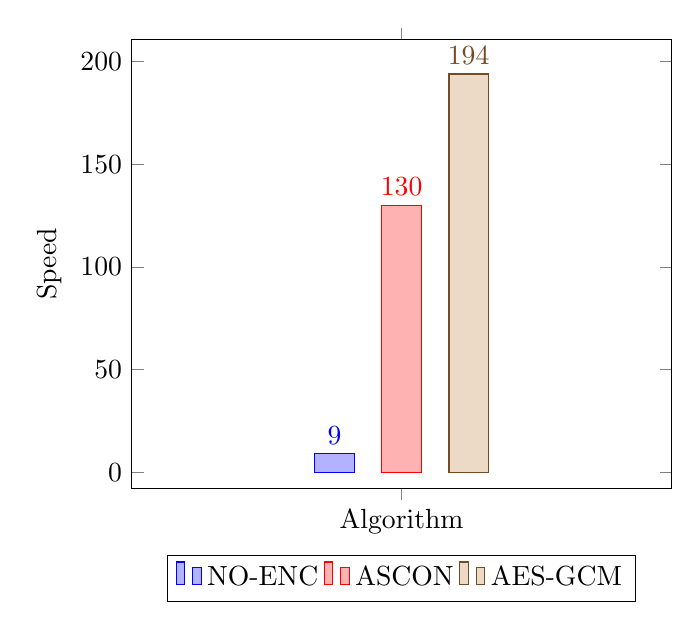
\begin{tikzpicture}
                    \begin{axis}[
                        ybar = 10pt,
                        enlargelimits=0.09,
                        legend style={at={(0.5,-0.15)},
                        anchor=north,legend columns=-1},
                        ylabel={Speed},
                        symbolic x coords={Algorithm, Scheme},
                        xtick=data,
                        nodes near coords,
                        nodes near coords align={vertical},
                        bar width = 0.5cm,
                        ]
                        \addplot coordinates {(Algorithm,9)};
                        \addplot coordinates {(Algorithm,130)};
                        \addplot coordinates {(Algorithm,194)};
                        % \addplot coordinates {(Algorithm,2)};
                         
                        \legend{NO-ENC, ASCON, AES-GCM}
                    \end{axis}
                \end{tikzpicture}
            }
        \caption{Speed From The Algorithm Execution Perspective.}
        \label{Fig:time-algorithm}
    \end{subfigure}%
    \begin{subfigure}[c]{0.48\linewidth}
        \resizebox{\linewidth}{!}{
            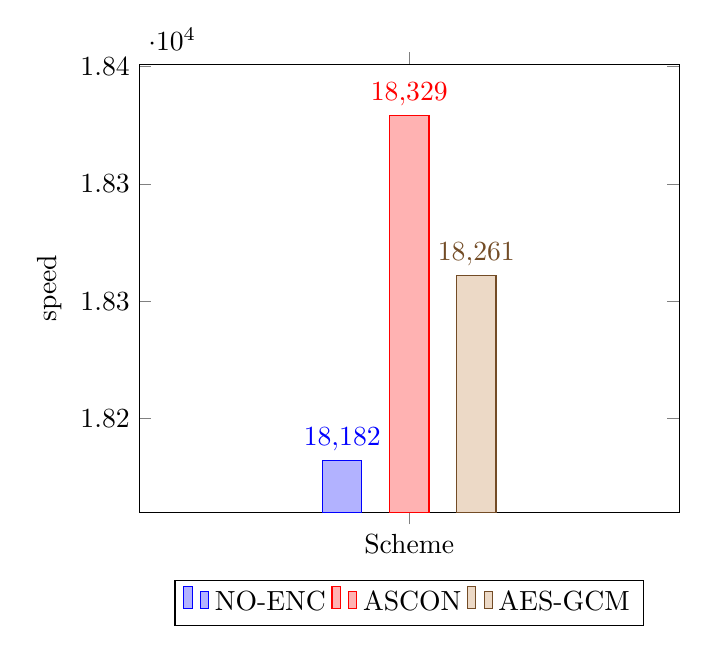
\begin{tikzpicture}
                \begin{axis}[
                    ybar = 10pt,
                    enlargelimits=0.15,
                    legend style={at={(0.5,-0.15)},
                    anchor=north,legend columns=-1},
                    ylabel={speed},
                    symbolic x coords={Scheme},
                    xtick=data,
                    nodes near coords,
                    nodes near coords align={vertical},
                    bar width = 0.5cm,
                    ]
                    \addplot coordinates {(Scheme,18182)};
                    \addplot coordinates {(Scheme,18329)};
                    \addplot coordinates {(Scheme,18261)};
                    % \addplot coordinates {(Algorithm,2)};
                     
                    \legend{NO-ENC, ASCON, AES-GCM}
                \end{axis}
            \end{tikzpicture}
            }
    \caption{Speed From The Scheme (Application) Perspective.}
    \label{Fig:time-scheme}
\end{subfigure}
\caption{Sample of how to use subfigures.}
\label{Fig:Theo_SFDev}
\end{figure}

\subsubsection*{Throughput and Cycle Byte Ratio}

Throughput is a performance indicator of a system that measures the number of bytes processed per unit of time (typically seconds). It is a measure of how efficiently a system can process data. The more bytes that are processed per unit of time, the better the system performs. Throughput is typically measured in bytes per second (Bps) or kilobytes per second (Kbps).

The Cycle Byte Ratio is another performance metric that measures the number of CPU cycles needed to process a single byte. Table \ref{tbl:cycle-count} presents the cycle counts for different scenarios: 1) without employing any encryption algorithm, 2) utilizing the ASCON encryption algorithm, and 3) employing the AES-GCM encryption algorithm.


\begin{table}[H]
    \centering
    \caption{Cycle Count For 3 Cases: No-Encryption, ASCON, AES-GCM }
    \label{tbl:cycle-count}
    \resizebox{\textwidth}{!}
    {
        \begin{tabular}{l | a | b | a}
        \hline
        \rowcolor{LightCyan}
        \mc{1}{}  & \mc{1}{No-Encryption}  & \mc{1}{ASCON} & \mc{1}{AES-GCM}\\
        \hline
        Cycle Count & 2009 & 36811  &  49956\\
        Byte Processed & 32  & 32 &  32\\ 
        CPU Freq MHz & 240 & 240 &  240\\ 
        Cycle per Byte &  64.28 & 1094.68 &  31517.90\\ 
        Time Elapsed $\mu$s & 8.57  & 145.95 &  202.38\\ 
        Throughput B/$\mu$s & 3.73  & 0.219 &  0.158\\ 
        \hline
        \end{tabular} 
        }
\end{table}

\begin{equation}
\text{Throughput} = \frac{\text{Byte processed}}{\text{Total Time}} \quad \text{Cycle Byte} = \frac{\text{Cycle Count}}{\text{Byte processed}}
\end{equation}

The total time taken by the CPU to perform an operation can be derived using cycle count and the CPU clock frequency. The total time taken by the operation is equal to the cycle count multiplied by the CPU clock frequency. 

To calculate the throughput and the cycle byte ratio for each algorithm in our proposed solution, we use 64 bytes of data as input. The summarized statical data is provided in Figure \ref{fig:per-cb}

\begin{equation}
\text{Total Time} = \frac{\text{Cycle Count}}{\text{CPU frequency in Mhz/Khz}}
\end{equation}

In this experiment, while we use \texttt{$xthal\_get\_ccount()$} from esp32/ck.h library to get the cycle count at a given time, we use \texttt{$getCpuFrequencyMhz()$} function to get the current set CPU frequency of the device fro esp32-hal-cpu.c source file.  

We calculated the throughput and cycle byte ratio of each algorithm in the proposed solution processing 16 bytes of message and 16 bytes of associated data, using equation (4.1). The results are shown in Figures \ref{fig:put} and \ref{fig:ccb-ratio}.


\begin{figure}[H]
        % \centering
        \begin{subfigure}[c]{0.48\linewidth}
            \resizebox{\linewidth}{!}{
                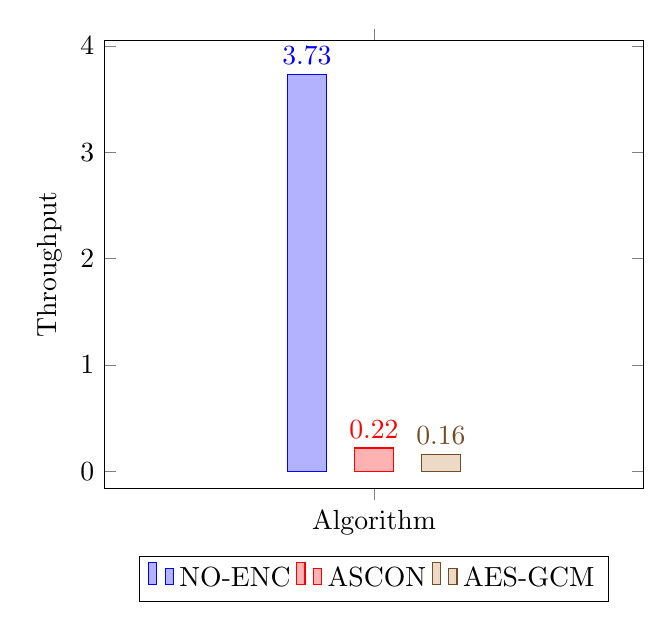
\begin{tikzpicture}
                    \begin{axis}[
                        ybar = 10pt,
                        enlargelimits=0.09,
                        legend style={at={(0.5,-0.15)},
                        anchor=north,legend columns=-1},
                        ylabel={Throughput},
                        symbolic x coords={Algorithm},
                        xtick=data,
                        nodes near coords,
                        nodes near coords align={vertical},
                        bar width = 0.5cm,
                        ]
                        \addplot coordinates {(Algorithm,3.73)};
                        \addplot coordinates {(Algorithm,0.219)};
                        \addplot coordinates {(Algorithm,0.158)};
                         
                        \legend{NO-ENC, ASCON, AES-GCM}
                    \end{axis}
                \end{tikzpicture}
            }
        \caption{Throughput of the algorithms.}
        \label{Fig:put}
    \end{subfigure}%
    \begin{subfigure}[c]{0.48\linewidth}
        \resizebox{\linewidth}{!}{
            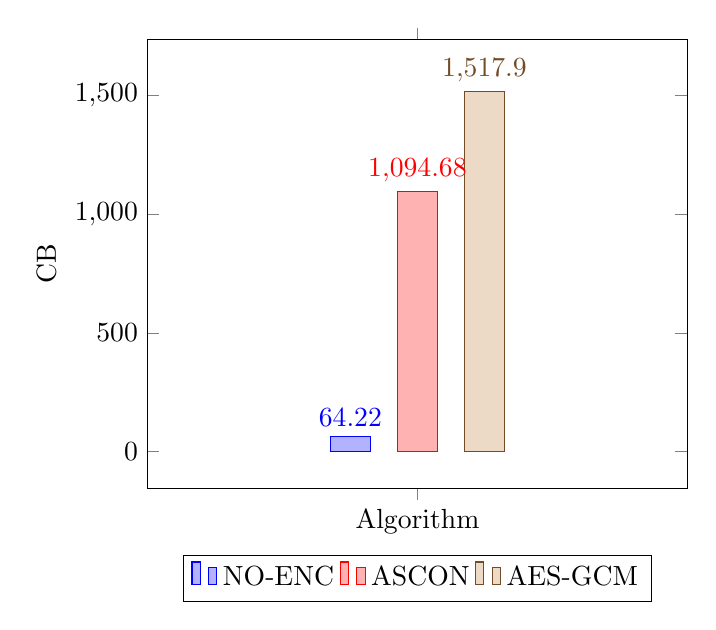
\begin{tikzpicture}
                \begin{axis}[
                    ybar = 10pt,
                    enlargelimits=0.15,
                    legend style={at={(0.5,-0.15)},
                    anchor=north,legend columns=-1},
                    ylabel={C\\B},
                    symbolic x coords={Algorithm},
                    xtick=data,
                    nodes near coords,
                    nodes near coords align={vertical},
                    bar width = 0.5cm,
                    ]
                    \addplot coordinates {(Algorithm,64.218)};
                    \addplot coordinates {(Algorithm,1094.68)};
                    \addplot coordinates {(Algorithm,1517.90)};
                    % \addplot coordinates {(Algorithm,2)};
                     
                    \legend{NO-ENC, ASCON, AES-GCM}
                \end{axis}
            \end{tikzpicture}
            }
    \caption{Cycle per Byte ratio.}
    \label{Fig:ccb-ratio}
\end{subfigure}
\caption{Throughput and cycle per byte ratio of each algorithms.}
\label{Fig:Theo_SFDev}
\end{figure}


% ****************************************************************************************
\subsection{Static and Dynamic Memory Footprint }
% show the ram and flash memory of embeded progrma 
Analyzing and measuring the memory usage of embedded programs is vital, especially when the device has memory constraints. In this section, we will discuss the static and dynamic memory usage of our proposed solution. Throughout our measurement,  compared three implementations scenarios:
\begin{itemize}
    \item No encryption,
    \item Encryption using ASCON, and
    \item Encryption using AES-GCM
\end{itemize}



\begin{figure}[H]
    \centering
    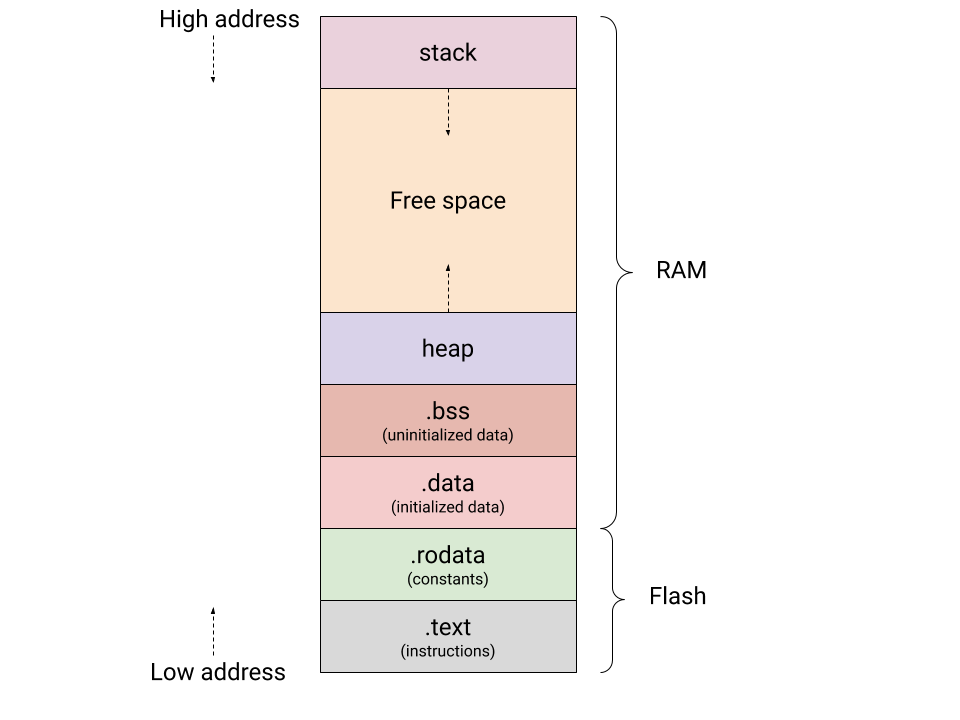
\includegraphics[width=\linewidth]{images/fp/memory-analysis.png}
    \caption{Memory Map of Embedded Programming \cite{alcarazDigitalTwinComprehensive2022}}
    \label{fig:memory-map}
\end{figure}

Figure \ref{fig:memory-map} depicts the general memory map of embedded programming. The flash part of the memory that includes the .rodata and .text section contains the code resulting from compiling and building the source program. This section contains static codes and requires a fixed memory size. Whereas, the RAM section of the memory is responsible for containing a few sections for statically generated codes and the majority one for handling dynamic memory management such as stack and heap allocation.


In our analysis of the dynamic memory usage for our implementation of the proposed solution, we focused only on the RAM section. However, when assessing the static memory usage (code size), we examined both the RAM and Flash sections. This approach was necessary as both sections contribute to the overall code size. 

\subsubsection{Static Memory Usage - Code size}
% Provide a table 
% Draw a graph 

The static code size measurement was conducted to compare the code size requirements of three different implementation scenarios: No-Encryption, ASCON, and AES-GCM. The goal was to assess the impact of these implementations on resource-constrained devices in terms of memory usage.

Table \ref{tbl:ins-codesize} provides a summary of the code size measurements for each scenario. In the No-Encryption scenario, no additional code was required beyond the base program, resulting in minimal memory usage. Our implementation based on ASCON introduced a slight increase in code size. Approximately 1 KB of additional memory was needed in both RAM and Flash compared to the No-Encryption scenario. On the other hand, AES-GCM demonstrated slightly higher code size requirements. The implementation demanded approximately 8 KB more RAM and 5.6 KB more Flash memory compared to the No-Encryption case.


\begin{table}[H]
    \centering
    \caption{Code Size: No-Encryption, ASCON, AES-GCM }
    \label{tbl:ins-codesize}
    \resizebox{\textwidth}{!}
    {
        \begin{tabular}{l | a | b | a}
        \hline
        \rowcolor{LightCyan}
        \mc{1}{}  & \mc{1}{No-Encryption}  & \mc{1}{ASCON} & \mc{1}{AES-GCM}\\
        \hline
        Ram \/KB & 59.3 & 59.3  &  68\\
        Flash & 766.5  & 767.7 &  772.1\\ 
        Total & 825.8 & 827 &  840.1\\ 
        % Cycle per Byte &  64.28 & 1094.68 &  31517.90\\ 
        % Time Elapsed $\mu$s & 8.57  & 145.95 &  202.38\\ 
        % Throughput B/$\mu$s & 3.73  & 0.219 &  0.158\\ 
        \hline
        \end{tabular} 
        }
\end{table}

\begin{figure}[H]
    \centering
    \caption{Static Code Size of The Scheme For 3 Scenarios(No-Encryption, ASCON, AES-GCM}
    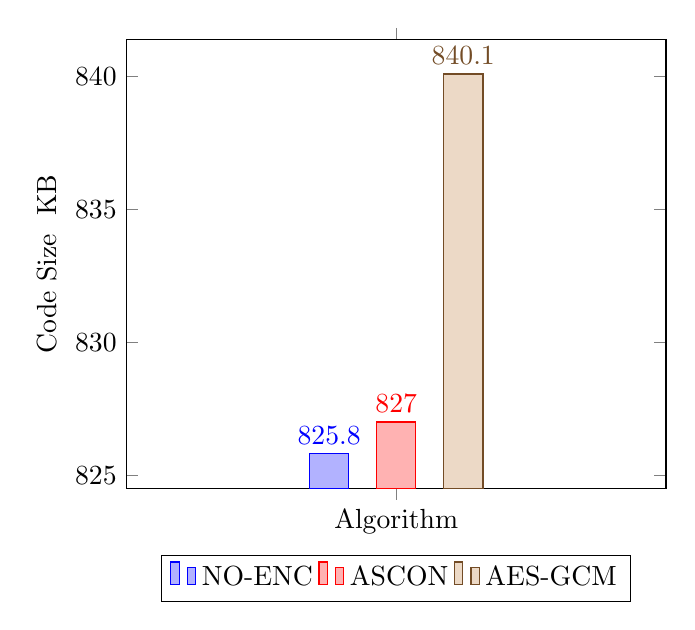
\begin{tikzpicture}
        \begin{axis}[
            ybar = 10pt,
            enlargelimits=0.09,
            legend style={at={(0.5,-0.15)},
            anchor=north,legend columns=-1},
            ylabel={Code Size \/ KB},
            symbolic x coords={Algorithm},
            xtick=data,
            nodes near coords,
            nodes near coords align={vertical},
            bar width = 0.5cm,
            ]
            \addplot coordinates {(Algorithm,825.8)};
            \addplot coordinates {(Algorithm,827)};
            \addplot coordinates {(Algorithm,840.1)};
             
            \legend{NO-ENC, ASCON, AES-GCM}
        \end{axis}
    \end{tikzpicture}    
\label{Fig:codesize}
\end{figure}

\subsubsection{Dynamic RAM Usage}

% I will explain the techniques I used to capture the memory usage
% The challenge of measuring the memory heap 
% Explain or provide an analysis of memory for each case 

Measuring the dynamic RAM usage of each algorithm is not as easy as measuring static memory usage. The heap and stack are two types of dynamic memory, making it challenging to keep track of their usage as they are allocated and freed during function calls and returns. One effective technique recommended by NIST is to overwrite the memory with known values before running the program and keeping track of the memory cells that are overwritten by the program [ref]. However, due to the complexity of setting it up,  we decided to employ alternative techniques to approximate the dynamic memory usage of each algorithm described as follows.



In our device (ESP32), we discovered that the initially allocated memory for handling heap and stack allocation is 327,680 Bytes. Having this in mind, we tracke the minimum heap size ever available, utilising the system call \textit{esp\_get\_minimum\_free\_heap\_size}. Our program was executed for 1000 iterations calling the encryption function for each implementation, allowing us to obtain a snapshot of the free memory available between the stack and heap 1000 times. By calculating the difference between the total allocated dynamic memory and the minimum heap size recorded, we were able to approximate the memory footprint of each implementation.

Furthermore, we employed the baseline implementation, which does not incorporate an encryption/decryption algorithm, as a benchmark to estimate the dynamic memory usage overhead added by ASCON and AES-GCM algorithms(see Fig \ref{Fig:memory-algo}). This comparison with the baseline provided insight into the dynamic memory usage of each algorithm at the running time. 

\begin{figure}[H]
        \caption{Dynamic Memory Usage Comparison of Our Scheme Implementation and Algorithms}
        % \centering
        \begin{subfigure}[c]{0.48\linewidth}
            \caption{Heap and Stack Memory Usage Each Implementation.}
            \resizebox{\linewidth}{!}{
                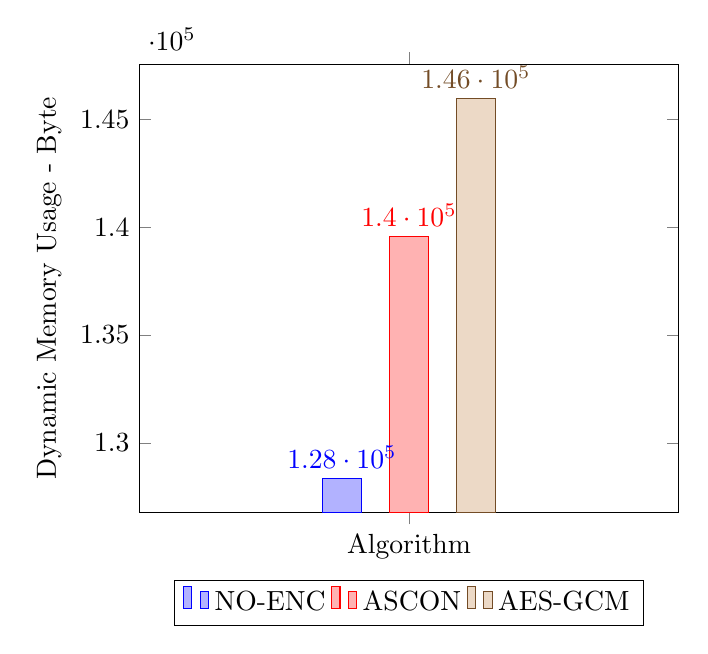
\begin{tikzpicture}
                    \begin{axis}[
                        ybar = 10pt,
                        enlargelimits=0.09,
                        legend style={at={(0.5,-0.15)},
                        anchor=north,legend columns=-1},
                        ylabel={Dynamic Memory Usage - Byte},
                        symbolic x coords={Algorithm},
                        xtick=data,
                        nodes near coords,
                        nodes near coords align={vertical},
                        bar width = 0.5cm,
                        ]
                        \addplot coordinates {(Algorithm,128356)};
                        \addplot coordinates {(Algorithm,139588)};
                        \addplot coordinates {(Algorithm,145972)};
                         
                        \legend{NO-ENC, ASCON, AES-GCM}
                    \end{axis}
                \end{tikzpicture}
            }
        \label{Fig:dynamic-memory}
    \end{subfigure}%
    \begin{subfigure}[c]{0.48\linewidth}
        \caption{The Additional Memory Overhead Introduced by the Algorithm.}
        \resizebox{\linewidth}{!}{
            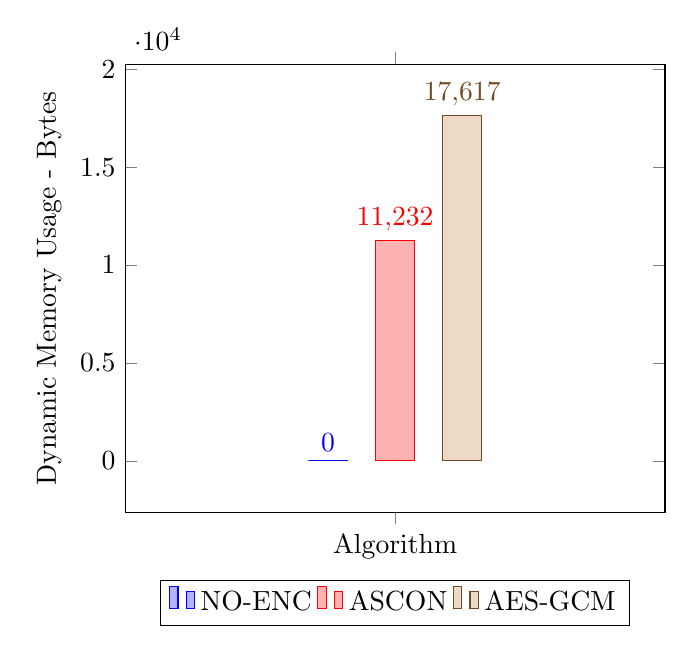
\begin{tikzpicture}
                \begin{axis}[
                    ybar = 10pt,
                    enlargelimits=0.15,
                    legend style={at={(0.5,-0.15)},
                    anchor=north,legend columns=-1},
                    ylabel={Dynamic Memory Usage - Bytes},
                    symbolic x coords={Algorithm},
                    xtick=data,
                    nodes near coords,
                    nodes near coords align={vertical},
                    bar width = 0.5cm,
                    ]
                    \addplot coordinates {(Algorithm,0)};
                    \addplot coordinates {(Algorithm, 11232)};
                    \addplot coordinates {(Algorithm, 17617)};
                    % \addplot coordinates {(Algorithm,2)};
                     
                    \legend{NO-ENC, ASCON, AES-GCM}
                \end{axis}
            \end{tikzpicture}
            }
    \label{Fig:memory-algo}
\end{subfigure}
\label{Fig:memory-impl-algo}
\end{figure}

\subsection{Power Consumption Measurement }


\section{Security Analysis of ASCON}
\textit{Preliminary assumption:} The proposed scheme in this paper uses the Ascon algorithm, which provides 128-bit security. As long as the security of Ascon is not broken, the proposed scheme is secure. The only information leaked to the adversary is the associated data, namely the thing ID (id). This information does not give any advantage to an attacker. The thing ID (id) is the additional data (or associated data ) in our authenticated encryption implementation. Furthermore, we assume that the private (symmetric) key employed for communication purposes is deployed before the communication starts through some sort of secure communication. 


However, it is important to note that the application protocol used, specifically the MQTT protocol, is not encapsulated or secured using TLS or any other security protocol. As a result, all the metadata associated with the MQTT protocol is openly available to the public.